% !TeX root = ../main.tex
% -*- coding: utf-8 -*-

\chapter{初始近边界数据的生成}\label{3}

目前,大多数模型的知识产权保护方法采用模型水印和模型指纹等被动防御方式来进行所有权验证,这种方式很难抵御歧义攻击。数据集推断利用训练数据在模型上的最优性进行所有权决策,从而验证所有权,但要求训练数据私有,因此应用范围小且推广难度高。因此,本文提出了一种数据驱动的推断模型所有权的新思路,该方法利用数据在模型上的最优性来推断模型所有权,代替传统的水印和指纹验证模型所有权,可以有效避免歧义攻击。同时,本文通过构造一种特殊的数据代替训练数据来推断模型所有权,使得训练数据可以被公开。

\section{模型所有权验证的局限性}\label{3.1}

现有的模型知识产权保护措施着重于被动的防御,只考虑针对模型修改的抗攻击性。模型所有者将水印嵌入训练好的模型或从其中提取抽象的模型知识作为指纹。如果怀疑一个模型的知识来自于源模型,模型所有者可以利用水印或指纹被动地从外部验证模型所有权,当检测到相应的水印或者指纹相匹配就代表该模型是从源模型派生。大多数工作基于这样的思路,设计不同的水印和指纹用于在源模型被盗窃后验证模型所有权,但这并不具备较强的鲁棒性。嵌入水印对源模型性能和功能的影响和需要的的额外代价都是模型水印研究工作的关键点。模型指纹目的是提取代表模型知识的固有特征,相较于水印指纹不会对源模型产生影响,因为模型的知识是容易被修改,因此指纹是脆弱的,所有的指纹方法都试图找到可以承受某些修改攻击的强鲁棒性指纹。

本文的目标不仅是抵御一般的模型窃取攻击,还集中在水印和指纹另一个亟待解决的问题歧义攻击上。歧义攻击不关心如何去除水印和指纹以通过模型所有权验证,而是通过伪造额外的水印和指纹混淆所有权验证。

如图\ref{歧义攻击示意图}所示,为了保护自己的知识产权,模型所有者在训练完源模型后,给DNN模型嵌入水印,然后发布模型提供公开服务。模型盗窃者访问公开的模型或者模型所提供的服务API,通过一定的方法复制篡改而得到盗版模型。为了躲避模型所有者的检测,盗窃者不关心原有的水印,而是给模型嵌入自己的额外水印。模型指纹的歧义攻击与水印类似,盗窃者不关注原有的指纹,而是提取新的指纹,以此混淆模型所有权的验证。

\begin{figure}[htb]%%图,[htbp]是浮动格式
	\centering
	%	\setlength{\abovecaptionskip}{2mm} %图片标题与图片距离
	\vspace{-2mm}
	\setlength{\belowcaptionskip}{-3mm} %调整图片标题与下文距离
	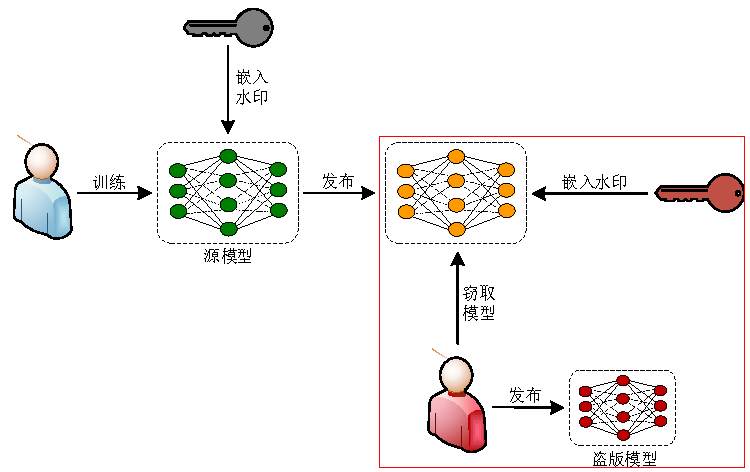
\includegraphics[width=0.9\linewidth]{歧义攻击示意图.pdf}
	\caption{歧义攻击示意图}
	\label{歧义攻击示意图}
	%	\vspace{-3mm}  %调整图片标题与下文距离,与\setlength{\belowcaptionskip}{-3mm}等效。
\end {figure}	

如图\ref{检测歧义示意图}所示,如果模型所有者怀疑可疑模型是从自己的源模型派生,向官方机构发起仲裁。仲裁机构进行模型所有者的水印或指纹检测,成功检测到嵌入的水印或成功匹配指纹。而于此同时,盗窃者的水印或指纹同样能够被仲裁机构所验证,这种情况下无法进行正确的所有权决策。直觉上,直觉上,如果模型盗窃者可以在水印模型上嵌入第二个水印或者提取第二个指纹,那么该模型的所有权归属存在巨大的歧义。

\begin{figure}[htb]%%图,[htbp]是浮动格式
	\centering
	\setlength{\abovecaptionskip}{3mm} %图片标题与图片距离
	%	\vspace{-2mm}
	\setlength{\belowcaptionskip}{-3mm} %调整图片标题与下文距离
	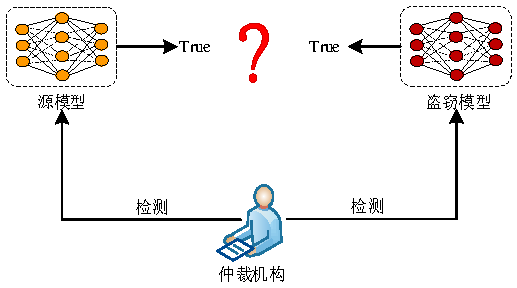
\includegraphics[width=0.6\linewidth]{检测歧义示意图.pdf}
	\caption{检测歧义示意图}
	\label{检测歧义示意图}
	%	\vspace{-3mm}  %调整图片标题与下文距离,与\setlength{\belowcaptionskip}{-3mm}等效。
\end {figure}

盗窃者对源模型嵌入新的水印或提取其他的指纹使原本的保护措施无效,歧义攻击对现有的深度神经网络模型的知识产权保护方法构成了严重威胁,在传统的数字水印领域中有研究表明,除非水印方案是不可逆的\cite{fan2019rethinking},否则鲁棒性的水印也不一定能验证所有权。

本文认为通过验证可疑模型是否具有源模型特定的水印或指纹来讨论盗窃行为是不充分的,特别是出现歧义攻击时,容易产生所有权混淆。因此本文提出推断模型所有权而不是验证,这是一种解决DNN模型所有权问题的新思路,与传统的通过模型水印和指纹验证所有权有所不同。这种方法是受数据集推断\cite{maini2021dataset}提出的数据驱动决策所有权的启发,利用某类数据在源模型上的最优性推断模型所有权,在下一小节中将具体讨论。


\section{模型所有权推断}\label{3.2}

数据集推断做了一个假设:源模型的知识来自于训练数据集。无论盗窃模型是直接攻击源模型还是其副产品,盗窃模型的知识仍然是源模型中包含的知识。如果原始训练数据集是私有的,那么模型所有者在进行数据集推断时,相比盗窃者拥有强大的优势,因为源模型在原始训练数据中的性能要远远优于其他数据集。因此,模型所有者通过评估多个数据点到分类边界的距离和统计测试相结合,可以得到模型的所有权归属。这种方式与模型水印和指纹验证所有权的方式有着本质的区别,该方式并不是去验证特定的水印或指纹,而是比较某类数据在模型上的最优性。

如图\ref{数据集推断原理图}所示,因为DNN模型是从数据集训练而来,所以模型中总会包含来自数据集中的知识。盗窃模型是从源模型派生,尽管包含的知识和源模型不可能完全相同,但总是有一部分是来自原始数据集,这是利用数据集做模型所有权推断的理论基础。

\begin{figure}[htbp]%%图,[htbp]是浮动格式
	\centering
	\setlength{\abovecaptionskip}{3mm} %图片标题与图片距离
	%	\vspace{-2mm}
	\setlength{\belowcaptionskip}{-3mm} %调整图片标题与下文距离
	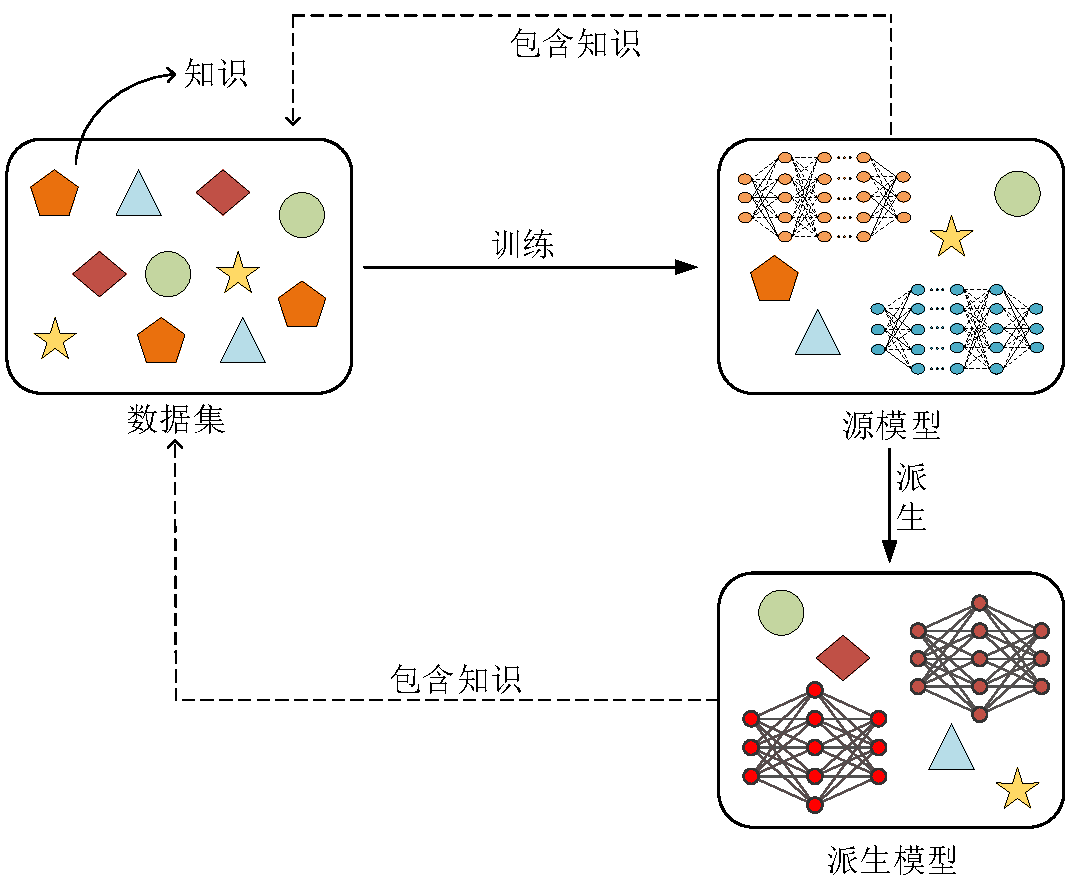
\includegraphics[width=0.8\linewidth]{数据集推断原理图.pdf}
	\caption{数据集推断原理图}
	\label{数据集推断原理图}
	%	\vspace{-3mm}  %调整图片标题与下文距离,与\setlength{\belowcaptionskip}{-3mm}等效。
\end {figure}	

模型窃取过程中,源模型中的知识会传播到盗窃模型,使得所有盗窃模型总是包含一部分源模型训练数据集中的直接或间接信息。利用数据集做模型所有权推断和传统的验证模型所有权不同,通过私有数据集推断得到的是一个所有权决策,其中决策的最大者被认为拥有所有权。传统的模型所有权验证是从模型中提取水印或指纹进行匹配从而验证,这种方式容易受到歧义攻击,进而导致的验证冲突。从决策过程可以发现数据集推断得到的是一个“最”的概念,模型的所有权归属于决策指标的最大者,而不是进行类似模型水印和指纹的特定响应匹配,因此可以有效避免歧义攻击。

本文的工作是受到数据集推断验证模型所有权的启发,使用数据驱动推断模型所有权代替验证模型所有权。所有权推断可以在有效证明所有权归属的同时,解决所有权验证冲突的问题。除此之外,数据驱动的推断所有权意味着该方法只和DNN模型的输入输出相关,那么数据驱动推断模型所有权的方法既可以在白盒环境也可以在黑盒环境下工作。

利用数据来推断模型所有权为保护模型知识产权提供了一个新的方向,但是目前数据集推断的方式仍然具有以下\textbf{局限性}:

1)使用数据集推断的前提是原始训练数据不能被盗窃者获得,所以公开的数据集不能被用于训练源模型。然而,在大多数真实场景下,只有很少一部分工作会构造私有数据集用于训练模型,甚至这部分工作只应用于特定的领域中,这也意味着模型被盗窃的风险较小。因此,依赖于私有数据集的数据集推理方法在实际应用中使用范围很小,不能被大幅度推广使用。

2)数据集推断方法的核心思想是源模型的功能在训练数据上的效果优于其他数据,但是存在模型的功能可能相似,而结构和训练数据都不同的情况,因此该方法的结果可能会导致错误,将不相关模型判定为盗窃模型。Li等人\cite{lao2022deepauth}验证了这个局限性,表明在此种情况下该方法产生的结果值得怀疑。

因此,亟需一种模型知识产权保护方法,在能成功判断模型所有权归属的同时,解决歧义攻击问题,并且适用于公开数据集。本文提出的方法将基于近边界数据推断DNN分类模型所有权。


\section{初始近边界数据的生成}\label{3.3}

上一节提出使用数据驱动来推断模型所有权,为了使训练数据公开,本文需要寻找一种新的数据来代替训练数据进行推断。本节将介绍这种特殊的数据——近边界数据,并且研究生成近边界数据的算法。

\subsection{近边界数据的可继承性}

DNN分类器的主要目标是对输入数据样本进行分类,一个DNN分类器的特征通常由其决策模式和分类边界决定。然而,分类器的分类边界是一个抽象的概念,无法被具体表示,因此研究者一般通过某正常数据样本和对应生成的对抗性样本组成样本对用于反映分类边界。因为分类边界位于两者之间,所以一定规模的对抗样本对可以用于描述分类边界。由于无法以数学的方式直接定义分类边界,本文使用分类器的决策结果来反映分类边界。

在以往的研究中\cite{cao2021ipguard},可以使用分类边界作为模型指纹用于验证模型所有权。本文不使用分类边界作为模型指纹,而是基于分类边界构造一类特殊的数据用于推断模型所有权。本文称这类特殊的数据为近边界数据,下面给出本文近边界数据的定义:

\begin{Definition}[近边界数据]
	\label{def:1}
	给定数据样本$x$,阈值$\theta$,如果数据样本$x$满足$\vert g_i(x) - g_j(x) \vert \leq \theta$,其中$i \neq j $并且$min(g_i(x), g_j(x)) \geq \mathop{max} \limits_{k \neq i, j}g_k(x)$,$g_k(x)$代表数据样本$x$被决策为类别$k$的概率,则数据样本$x$被称为近边界数据。
\end{Definition}

近边界数据是指那些非常接近分类边界的数据样本,与位于分类边界上的数据样本类似,这些样本对模型的决策边界有重要的影响,因为它们能够揭示模型在分类边界附近的行为。由于近边界数据不要求样本完全位于分类边界上,因此即使模型受到修改,分类边界发生偏移,仍然可以衡量数据近边界性。所以相对于直接使用分类边界来作为模型指纹,近边界数据在面对模型窃取攻击时,有着更强的鲁棒性。

如图\ref{近边界数据示意图}所示,近边界数据位于DNN分类器的分类边界附近,其他数据的分布则离分类边界较远。判定是否为近边界数据由定义\ref{def:1}中的阈值$\theta$决定,当$\theta$较小时,近边界数据样本表现为更加靠近模型分类边界。

\begin{figure}[htbp]%%图,[htbp]是浮动格式
	\centering
	\setlength{\abovecaptionskip}{5mm} %图片标题与图片距离
	%	\vspace{-2mm}
	\setlength{\belowcaptionskip}{-3mm} %调整图片标题与下文距离
	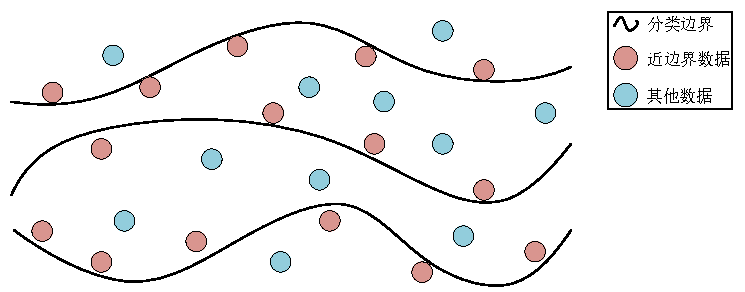
\includegraphics[width=0.9\linewidth]{近边界数据示意图.pdf}
	\caption{近边界数据示意图}
	\label{近边界数据示意图}
	%	\vspace{-3mm}  %调整图片标题与下文距离,与\setlength{\belowcaptionskip}{-3mm}等效。
	\end {figure}
	
在\ref{5}\ref{5.4}中,本文通过大量的实验验证了近边界数据在大多数的模型窃取技术中其近边界特征被保留,表明近边界数据的近边界性可以很好的继承到源模型派生出的模型上。因此,近边界数据可以作为推断所有权的依据被使用。尽管近边界数据在模型的知识产权保护中表现出显著的效果,但是在实践中,获得一定规模的近边界数据样本仍然是一个具有挑战性的任务。这是因为自然的近边界数据在样本空间中的占比非常低,甚至可以被忽略不计。通常来说,寻找位于分类边界上的数据点采用重复随机采样数据点的方法,然而,简单的重复采样可能需要大量的时间消耗,甚至无法找到这样的数据点。因此,如何得到一定规模的近边界数据样本仍然是一个难题,生成近边界数据的过程将在下一节中详细介绍。

\subsection{初始近边界数据的生成}

根据最近的一些研究\cite{cao2021ipguard},对抗性样本通常被用于确定分类器的分类边界。具体而言,对抗性样本有两个分类:原始分类和目标分类。其中,原始分类是指该样本不经过特殊处理的原始分类结果,目标分类是对原始样本添加微小噪声后的分类结果。对抗性样本是通过向原始数据添加小量扰动或干扰来生成的,这些扰动通常很难被人眼察觉,但却足以改变DNN模型的分类结果。

如图\ref{原始样本与对抗性样本对比}所示,对抗性样本对分类边界的跨越体现在,在视觉上,对抗性样本和原始样本几乎没有差别,但是分类结果却完全不同,在有目标攻击的情况下,甚至可以人为的指定目标分类。

\begin{figure}[htb]%%图,[htbp]是浮动格式
\setlength{\abovecaptionskip}{3mm} %图片标题与图片距离
\vspace{-2mm}
\setlength{\belowcaptionskip}{-3mm} %调整图片标题与下文距离
\subfigure[原始样本]{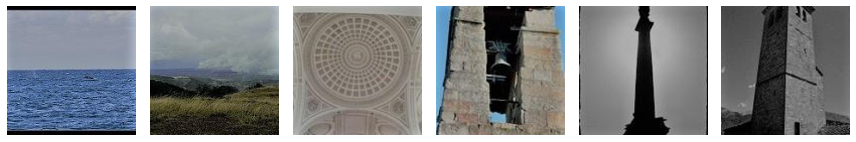
\includegraphics[width=1\linewidth]{原始样本.pdf}}
\subfigure[对抗性样本]{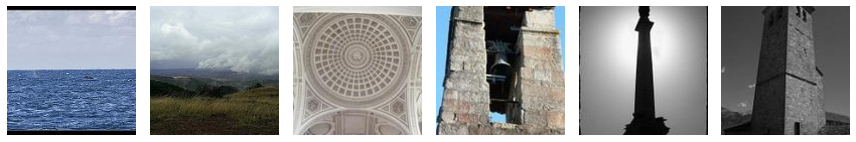
\includegraphics[width=1\linewidth]{对抗性样本.pdf}}
\caption{原始样本与对抗性样本的对比}
\label{原始样本与对抗性样本对比}
\end {figure}

对抗性样本会对模型分类边界进行跨越,本文认为该特征可以帮助获得较多的近边界数据。具体来说,本文将生成大量的对抗性样本,并从中挑选合适的近边界数据。因此,本文测试了几种常见的生成对抗性样本的方法,以帮助更好的构建近边界数据。因为本文需要数据样本尽可能靠近分类边界,因此在测试过程中,不同方法的优劣取决于生成对抗性样本到分类边界距离的远近,距离近者更优。

为了更好的衡量数据样本到分类边界的距离,在定义\ref{def:1}的基础上,下面给出量化的分类边界距离定义:

\begin{Definition}[分类边界距离]
	\label{def:2}
	给定一个数据样本$x$,它到分类边界的距离$distance = \vert g_i(x) - g_j(x) \vert$,其中$i \neq j $并且$min(g_i(x), g_j(x)) \geq \mathop{max} \limits_{k \neq i, j}g_k(x)$,$g_k(x)$代表数据样本$x$被决策为类别$k$的概率。
\end{Definition}

根据定义\ref{def:2},以分类边界距离为衡量标准,下面分别对几种常见的生成对抗性样本的方法进行介绍与测试。


\noindent\textbf{Fast \ Gradient \ Sign \ Method(FGSM):}FGSM \cite{goodfellow2014explaining}是最经典的生成对抗性样本的方法之一,它是一种基于梯度构建对抗性样本的方法,属于无目标的攻击方式。只需要对原始样本添加一次微小的扰动$\eta$,如式\ref{eq:3.1},\ref{eq:3.2}所示,即可生成样本$x$的对抗性样本$\tilde{x}$,十分高效。

\begin{equation}
	\setlength\abovedisplayshortskip{-5mm}
	%	 	\setlength\belowdisplayshortskip{4mm}
	\label{eq:3.1}
	\eta = \epsilon \cdot sign(\bigtriangledown_xJ(\theta,x,y^*))
\end{equation}
\begin{equation}
	\label{eq:3.2}
	\tilde{x} = clip(x + \eta)
\end{equation}

其中$sign$是符号函数,$x$表示原始样本,$y^*$表示$x$的真实类别,$\theta$表示模型权重参数,$J$表示分类器损失函数,$\bigtriangledown_x$表示对原始样本$x$求偏导,$clip$函数是将样本投射回可行数据域,比如图像样本的像素点范围应该在$[0,1]$以内,$\epsilon$用来控制变化幅度大小。

FGSM 生成对抗性样本的速度非常快,但其结果非常依赖$\epsilon$的选择,因此探索不同的$\epsilon$是使用该方法的重点。

\noindent\textbf{Iterative \ Gradient \ Sign \ Method(IGSM):}IGSM\cite{kurakin2018adversarial}是FGSM的进阶版本,如式\ref{eq:3.3},\ref{eq:3.4}所示,与FGSM只进行一次扰动叠加不同,IGSM采用迭代的形式构造对抗性样本,每次叠加一个小扰动。这个过程持续到成功生成对抗性样本或者达到迭代次数上限为止。

\begin{equation}
	\setlength\abovedisplayshortskip{-5mm}
	\label{eq:3.3}
	\eta = \alpha \cdot sign(\bigtriangledown_xJ(\theta,x,y^*))
\end{equation}
\begin{equation}
	\label{eq:3.4}
	\tilde{x}_t = clip(\tilde{x}_{t - 1}  + clip_{\epsilon}(\eta))
\end{equation}

\noindent $\alpha$是步长大小,$\tilde{x}_t$表示第$t$次迭代后的结果,$clip_{\epsilon}$是限定每次叠加的范围不超过$\epsilon$,其余参数含义与FGSM保持一致。

除此之外,本文还测试了FGSM的另一个进阶版本RFSGM\cite{tramer2017ensemble},RFSGM增加了扰动的多样性,可以更精细地生成对抗性样本。在实际结果中,发现尽管FGSM生成对抗性样本速度非常快,但是对抗性样本距离分类边界的距离比较远。IGSM 和RFGSM 效果要比FGSM 好,但仍然没有达到本文的预期,生成的对抗性样本距离分类边界距离太远。在大量的测试中,本文发现CW能够生成大量位于分类边界附近的样本,具体的测试结果在\ref{5}\ref{5.2}中。

\noindent\textbf{Carlini \ and \ Wagner's \ methods(CW):}CW\cite{carlini2017towards}方法是一种有目标的攻击方式,与其他生成对抗性样本的方法类似,该方法是添加噪声到数据样本中,但其具有三种变体:CW-$L_0$,CW-$L_2$和CW-$L_{\infty}$。不同的变体使用不同的方法来衡量噪声的大小,其中CW-$L_2$在实验中生成对抗性样本的效果和生成效率相比其余两种变体较好,因此本文使用该方法作为生成对抗性样本的基础。具体而言,CW-$L_2$对于给定的初始样本,采用二分查找的方式来增大或减小式\ref{eq:3.7}中$c$,并且使用类似训练神经网络模型的方式来调整生成对抗性样本的其他参数。CW-$L_2$的损失函数和约束如式\ref{eq:3.5},\ref{eq:3.6},\ref{eq:3.7},\ref{eq:3.8}所示:
\begin{equation}
	%	\setlength\abovedisplayshortskip{-8mm}
	\label{eq:3.5}
	Loss = Loss1 + Loss2 
\end{equation}
\begin{equation}
	%	\setlength\abovedisplayshortskip{-8mm}
	\label{eq:3.6}
	Loss1 = D(x, x + \delta)
\end{equation}
\begin{equation}
	%	\setlength\abovedisplayshortskip{-5mm}
	\label{eq:3.7}
	Loss2 = c \cdot f(x + \delta,target)
\end{equation}
\begin{equation}
	%	\setlength\abovedisplayshortskip{-5mm}
	%	\setlength\belowdisplayshortskip{-3mm}
	\label{eq:3.8}
	x + \delta \in [0,1]^m
\end{equation}

其中$target$是生成对抗性样本的目标标签,$c$是惩罚因子,用于权衡$Loss2$的影响大小,算法通过二分查找来寻找合适的$c$。$Loss1$约束对抗性样本$x + \delta$和原始样本$x$尽可能相似,$Loss2$约束对抗性样本$x + \delta$的决策结果为目标标签,式\ref{eq:3.8}约束对抗性样本在正常的图像范围内。

\begin{algorithm}[H] 
	\setstretch{1.2}
	\small
	\caption{\small 改进的二分查找CW-$L_2$算法}
	\label{alg:1}
	%	\small
	\begin{algorithmic}[1]
		\Require 样本$x$;模型$M$;阈值$\theta$;二分次数$n$;迭代次数$iteration$;原始标签$r$;目标标签$t$
		\Ensure 近边界对抗性样本$x'$
		\State 参数初始化:$c\gets1$,$distance \gets 1$
		\For {$i=1,2,...,n$}
		\State $isSuccessAttack \gets$ false
		\State $w \gets$ arctanh($x$)
		\State $w\_pert \gets$ zero\_like($w$)
		\For{$j=1,2,...,iteration$}
		\State $new\_img \gets$ tanh($w + w\_pert$)
		\State $new\_distance \gets\vert g_r(new\_img) - g_t(new\_img) \vert$
		\If{$new\_distance < distance$}
		\State $distance \gets new\_distance$
		\State $x' \gets new\_img$
		\State $isSuccessAttack \gets$ true
		\EndIf
		\State 使用Adam优化器更新$w\_pert$
		\EndFor
		\If{$isSuccessAttack$ == true}
		\State 减小$c$
		\Else \State 增大$c$
		\EndIf 
		\If{$distance \leq \theta$} 
		\State break
		\EndIf
		\EndFor
		\State \textbf{return} $x'$
	\end{algorithmic}
	
\end{algorithm}

根据定义\ref{def:2},数据样本$x$距离分类边界的距离是$distance = \vert g_i(x) - g_j(x) \vert$。本节的目标是生成的对抗性样本距离分类边界的距离尽可能近。本文在算法迭代过程中引入这一目标,以此改进算法迭代的过程,在使得生成对抗性样本更加靠近分类边界的同时,提高算法效率。具体而言,在迭代过程中,仅在$distance$变小时,更新距离参数和新生成的对抗性样本,并在$distance$小于等于预定的阈值$\theta$时,提前终止算法的迭代,具体的过程如算法\ref{alg:1}所示。





通过算法\ref{alg:1},本文已经可以生成大量位于分类边界附近的近边界数据。但是在这一阶段,本文只是在源模型的样本空间中挑选一部分数据作为初始样本添加微小噪声或扰动,针对性地生成了目标分类的对抗性样本。

在此阶段,源模型的训练和原始训练数据集均不受任何影响,防御者只需要针对性的生成对抗性样本即可。然而,近边界数据作为推断所有权的重要证据,直接生成对抗性样本也极易受到盗窃者的伪造。因此,本文需要将生成的近边界数据私有化,防止被盗窃者轻易伪造,具体操作将在下一节中给出。

\section{本章小结}

本章首先分析了现有的通过模型水印和模型指纹来做所有权验证的局限性,然后提出数据驱动的推断所有权的方法。鉴于近边界数据在源模型和其派生模型上的可继承性,本文使用近边界数据来代替训练数据进行所有权推断。由于自然的近边界样本很少,本文对比了主流的对抗性样本生成算法,根据生成样本到分类边界的距离。选择CW-$L_2$作为基础算法。并在此基础上改进,生成本文的初始近边界数据。